% Figure s01f05_selfconsistency (Session 1): the mean-field self-consistency loop, one pass computed.
% The image is rendered by figures/blender/s01f05_selfconsistency.py; the coordinates of the labels come from
% figures/blender/out/s01f05_selfconsistency_anchors.tex. Build with figures/blender/build_figure.sh s01f05_selfconsistency.
\documentclass[11pt,tikz,border=0pt]{standalone}
\usepackage[T1]{fontenc}
\usepackage{amsmath,amssymb,graphicx}
\usepackage{xcolor}
\usetikzlibrary{arrows.meta}
% The three label colors of the figures, with the same values as in src/figures_preamble.tex.
\definecolor{aqmaccent}{RGB}{31,78,121}
\definecolor{aqmbroken}{RGB}{168,42,34}
\definecolor{aqmmuted}{RGB}{125,125,125}

\newlength{\figw}\setlength{\figw}{16.63cm}   % 1.07 of the text width, before the empty margins of the render are cropped

\begin{document}
\begin{tikzpicture}[lbl/.style={font=\small, inner sep=1.5pt},
    flow/.style={line width=0.9pt, -{Stealth[length=5pt,width=4pt]}}]
  \node[overlay, anchor=south west, inner sep=0pt] at (0,0)
    {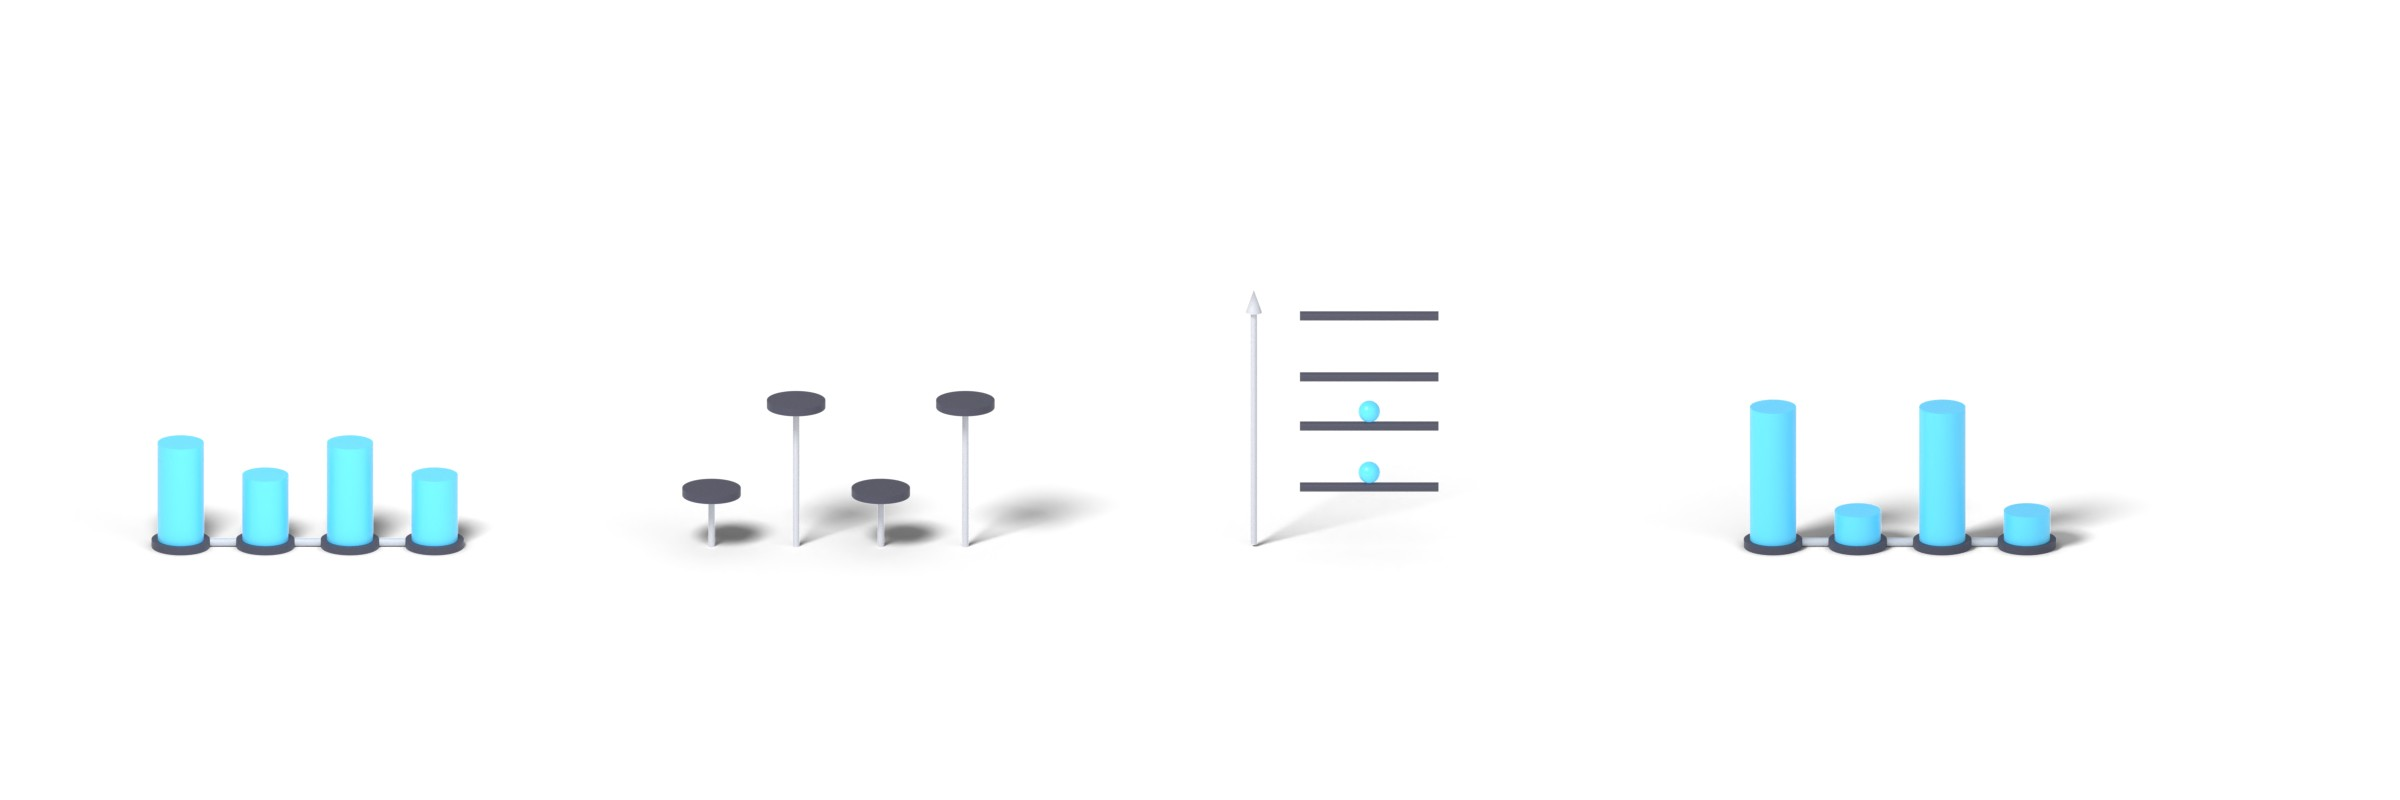
\includegraphics[width=\figw]{../blender/out/s01f05_selfconsistency.jpg}};
  % written by build_figure.sh; the painted part of the image
\path (0.0592\figw,0.0996\figw) rectangle (0.8883\figw,0.2125\figw);

  %% written by figlib.py; x and y in units of the image width
\coordinate (st1) at (0.1282\figw,0.2246\figw);
\coordinate (in1) at (0.0449\figw,0.1423\figw);
\coordinate (out1) at (0.2115\figw,0.1423\figw);
\coordinate (low1) at (0.1282\figw,0.0958\figw);
\coordinate (st2) at (0.3494\figw,0.2246\figw);
\coordinate (in2) at (0.2660\figw,0.1423\figw);
\coordinate (out2) at (0.4327\figw,0.1423\figw);
\coordinate (low2) at (0.3494\figw,0.0958\figw);
\coordinate (st3) at (0.5705\figw,0.2246\figw);
\coordinate (in3) at (0.4872\figw,0.1423\figw);
\coordinate (out3) at (0.6538\figw,0.1423\figw);
\coordinate (low3) at (0.5705\figw,0.0958\figw);
\coordinate (st4) at (0.7917\figw,0.2246\figw);
\coordinate (in4) at (0.7083\figw,0.1423\figw);
\coordinate (out4) at (0.8750\figw,0.1423\figw);
\coordinate (low4) at (0.7917\figw,0.0958\figw);

  \node[lbl, anchor=south, align=center] at (st1) {1.\ guess\\$\langle c_i^\dagger c_i\rangle$};
  \node[lbl, anchor=south, align=center] at (st2) {2.\ build\\$H_{\mathrm{MF}}$};
  \node[lbl, anchor=south, align=center] at (st3) {3.\ diagonalize,\\fill up to $N$};
  \node[lbl, anchor=south, align=center] at (st4) {4.\ recompute\\$\langle c_i^\dagger c_i\rangle$};
  \draw[flow] (out1) -- (in2);
  \draw[flow] (out2) -- (in3);
  \draw[flow] (out3) -- (in4);
  \draw[flow, aqmbroken] (low4) -- ++(0,-0.35cm) -| node[pos=0.25, below, lbl] {converged? no, repeat} (low1);
  \draw[flow, aqmaccent] (out4) -- ++(0.5cm,0) node[lbl, anchor=west, align=left] {yes\\solution};
\end{tikzpicture}
\end{document}
